\chapter{Risultati}
In questo capitolo vengono presentati i risultati degli esperimenti 
condotti. Il capitolo è diviso in tre sezioni.
Le prime due sezioni, una per dataset studiato, hanno la stessa 
struttura: il primo paragrafo sintetizza il 
setup dell'esperimento presentato e discute anche qualche esperimento
preliminare condotto che ha portato alla decisione di alcuni parametri.
In ultimo, la sezione finale discute possibili miglioramenti al setup
utilizzato in questo studio.


\section{FEMNIST}
In questa sezione vengono descritti gli esperimenti fatti con il dataset
FEMNIST e vengono descritti i risultati.

\subsection{Set up}
Come già anticipato, gli esperimenti sul dataset FEMNIST sono stati fatti 
utilizzando una CNN con 2 layer convoluzionali con 32 e 64 canali di 
output, seguiti da un layer lineare con 512 neuroni. Si sono provate le 
strategie di ibridazione \texttt{unify} e \texttt{share-disjoint},
condividendo i dataset selezionando alcuni client i cui dataset 
vengono interamente condivisi oppure prendendo una parte di sample da 
ogni dataset locale, mentre come gradi di ibridazione si è andati da 0\%,
completamente federato, al 100\%, completamente centralizzato,
in step di 10\%. Gli algoritmi di ottimizzazione provati sono SGD 
con learning rate \(\eta = 0.01\) e momentum \(\beta = 0.9\) e l'AdamW
con learning rate \(\eta = 0.01\). Il training ha usato 6 epoche locali
ed è durato per 20 round. Sono stati usati i sample di soltanto 100 
scrittori del totale presenti nel FEMNIST. I risultati presentati 
successivamente sono una media su 20 simulazioni.

Oltre ai risultati di questo esperimento, presentati nel paragrafo
successivo, sono stati fatte anche simulazioni preliminari con 
iperparametri diversi. Primo fra tutti è il numero di client, che negli 
esperimenti finali è stato mantenuto basso per velocizzare il processo 
di training, mentre sono state eseguite simulazioni fino a 1000 client 
utilizzati. Il numero poi stato mantenuto basso perché in tutti gli 
esperimenti fatti i risultati ottenuti erano sempre gli stessi, 
indipendentemente dal numero di client che partecipavano.
Un'altra risultato interessante è stato l'esperimento utilizzando SGD
senza momentum, in cui si è visto che la CNN non è riuscita a imparare,
mantenendo un accuracy sul dataset di test intorno al 6\%.

\subsection{Risultati}
Il dataset FEMNIST è quello dei due che si è dimostrato più difficile 
da imparare e su cui è più notevole il miglioramento di performance 
dato dalla condivisione dei dati (circa il 10\% dal setting totalmente
federato a quello totalmente centralizzato). La figura \ref{fig:femnistrandom}
mostra i risultati del training ai due estremi di ibridazione:
\ref{fig:femnistrandoma} mostra i risultati dell'apprendimento federato,
mentre \ref{fig:femnistrandomb} quelli dell'apprendimento centralizzato.
\begin{figure}[hb]  % h: here, t: top, b: bottom, p: page
    \centering
    \begin{subfigure}[b]{0.49\textwidth}
        \centering
        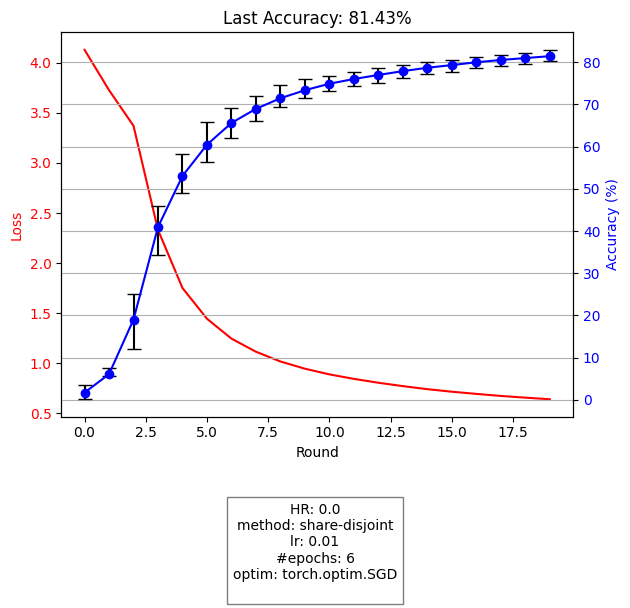
\includegraphics[width=\textwidth]{../plots/femnist-horizontal/sgd/results-h0_0-hm_share-disjoint-lr0_01-e6-torch_optim_SGD.png}
        \caption{Federato}
        \label{fig:femnistrandoma}
    \end{subfigure}
    \hfill
    \begin{subfigure}[b]{0.49\textwidth}
        \centering
        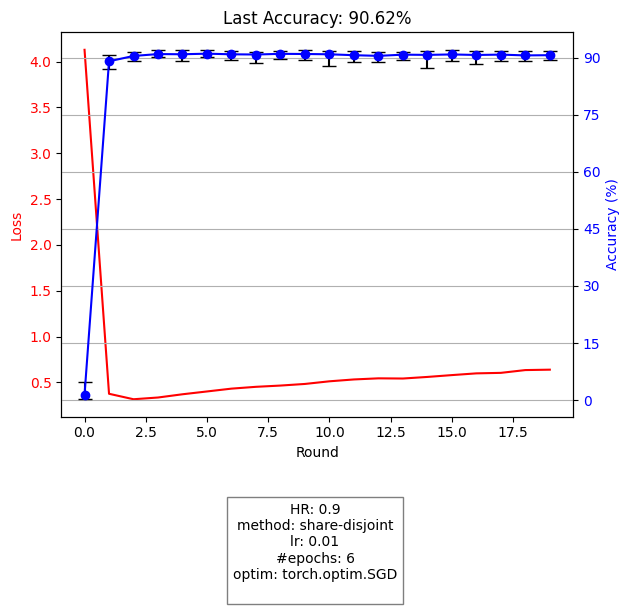
\includegraphics[width=\textwidth]{../plots/femnist-horizontal/sgd/results-h0_9-hm_share-disjoint-lr0_01-e6-torch_optim_SGD.png}
        \caption{Centralizzato}
        \label{fig:femnistrandomb}
    \end{subfigure}
    
    \caption{
        Risultati del del training per ogni round. A sinistra (a) si può 
        vedere l'apprendimento federato, a destra (b) quello centralizzato.
        Algoritmo di ottimizzazione (SGD) e metodo di condivisione 
        (\texttt{share-disjoint}) sono tenuti fissati.
    }
    \label{fig:femnistrandom}
\end{figure}


Come si può vedere nel caso federato 
le performance raggiungono una precisione del 81.43\% sul testset 
e si può anche notare che il modello non è ancora arrivato a convergenza.
Continuando il training per ulteriori round possiamo quindi aspettarci 
di poter migliorare le prestazioni ancora.
Il modello centralizzato arriva ad un'accuracy maggiore di un 9\% e 
soprattutto bastano 2 round per ottenere risultati sopra al 90\%.

Un primo caso di chiara convergenza intorno all'88\% lo si vede quando 
si inizia a condividere il 20\% dei dataset come mostrato in figura 
\ref{fig:femnists2sgd}, dove si può vedere che l'accuracy del modello 
smette di migliorare intorno al decimo round.
\begin{figure}[hb]  % h: here, t: top, b: bottom, p: page
    \centering
    \begin{subfigure}[b]{0.49\textwidth}
        \centering
        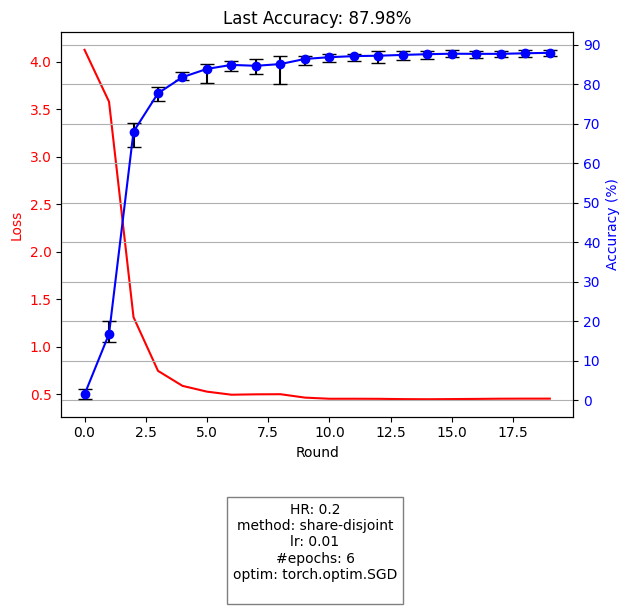
\includegraphics[width=\textwidth]{../plots/femnist-horizontal/sgd/results-h0_2-hm_share-disjoint-lr0_01-e6-torch_optim_SGD.png}
        \caption{\texttt{share-disjoint} con ibridazione 20\%}
        \label{fig:femnists2sgd}
    \end{subfigure}
    \hfill\begin{subfigure}[b]{0.49\textwidth}
        \centering
        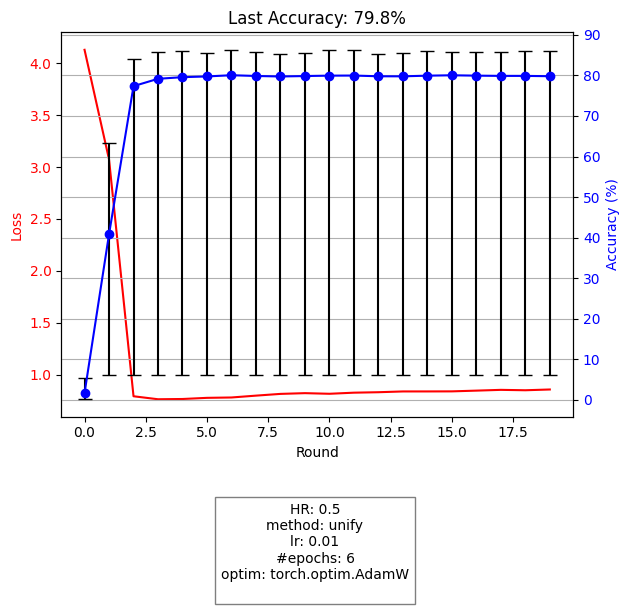
\includegraphics[width=\textwidth]{../plots/femnist-horizontal/adamw/results-h0_5-hm_unify-lr0_01-e6-torch_optim_AdamW.png}
        \caption{\texttt{unify} con ibridazione 50\%}
        \label{fig:feministu5adam}
    \end{subfigure}
    
    \caption{
        Risultati del training diversi. Il grafico a sinitra (a) 
        mostra i risultati di una condivisione \texttt{share-disjoint}
        al 20\%, mentre quello a destra (b) usa il metodo 
        \texttt{unify} al 50\%.
    }
    \label{fig:femnistadam}
\end{figure}

Dei due ottimizzatori provati, SGD è quello che performa meglio: è più 
veloce nell'apprendimento, ottiene performance migliori alla fine del 
training ed è molto più stabile. In particolare tutte le run che hanno 
utilizzato AdamW e il metodo di condivisione \texttt{unify} mostrano 
sempre intervalli di incertezza enormi, come quello riportato in 
figura \ref{fig:feministu5adam}. La situazione è analoga anche usando 
la condivisione \texttt{share-disjoint} fino a che il grado di 
condivisione non raggiunge un minimo del 40\%, come mostrato nelle 
figure \ref{fig:feminists3adam} e \ref{fig:feminists4adam}, e anche 
dopo oltre il 40\% non è garantita una maggiore stabilità, come ha 
rivelato l'esperimento con 80\% di condivisione (figura \ref{fig:feminists8adam}).
\begin{figure}[htbp]  % h: here, t: top, b: bottom, p: page
    \centering
    \begin{subfigure}[b]{0.49\textwidth}
        \centering
        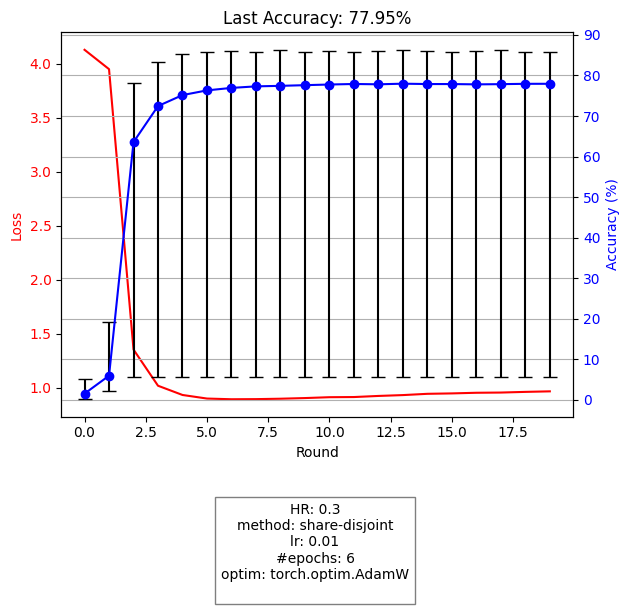
\includegraphics[width=\textwidth]{../plots/femnist-horizontal/adamw/results-h0_3-hm_share-disjoint-lr0_01-e6-torch_optim_AdamW.png}
        \caption{Figura 5.3(a)}
        \label{fig:feminists3adam}
    \end{subfigure}
    \hfill
    \begin{subfigure}[b]{0.49\textwidth}
        \centering
        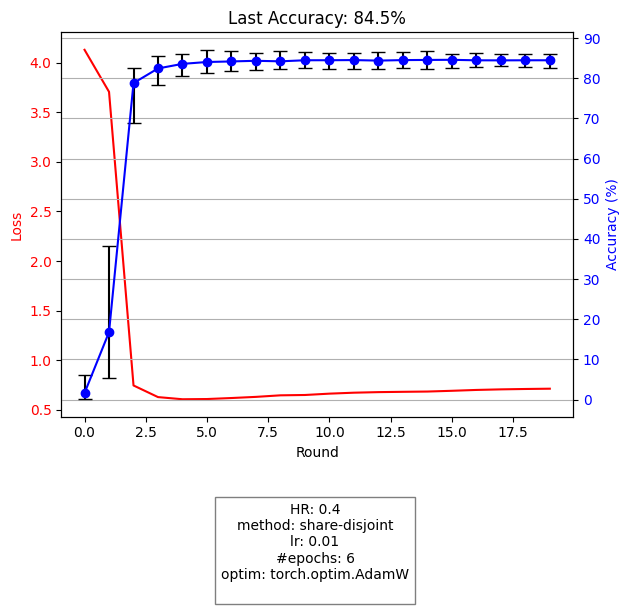
\includegraphics[width=\textwidth]{../plots/femnist-horizontal/adamw/results-h0_4-hm_share-disjoint-lr0_01-e6-torch_optim_AdamW.png}
        \caption{Figura 5.3(b)}
        \label{fig:feminists4adam}
    \end{subfigure}
    \centering
    \begin{subfigure}[b]{0.49\textwidth}
        \centering
        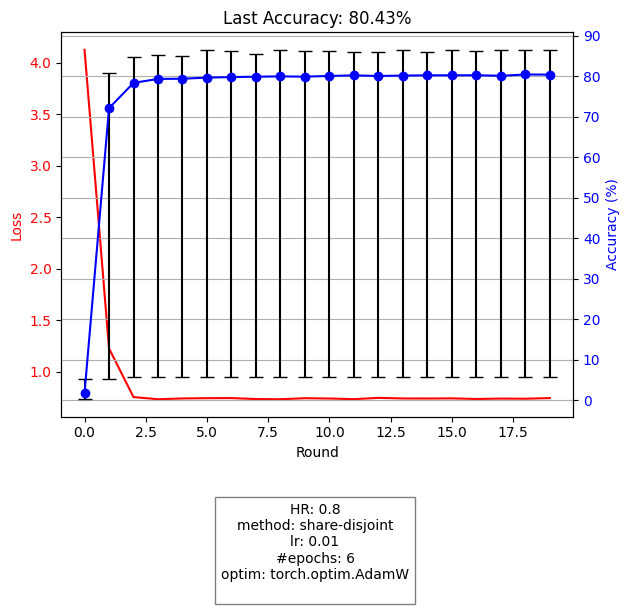
\includegraphics[width=\textwidth]{../plots/femnist-horizontal/adamw/results-h0_8-hm_share-disjoint-lr0_01-e6-torch_optim_AdamW.png}
        \caption{Figura 5.3(c)}
        \label{fig:feminists8adam}
    \end{subfigure}
    
    \caption{
        Diversi risultati di training con AdamW e metodo \texttt{share-disjoint}.
        Il primo (a) usa una condivisione del 30\%, il secondo (b) al 40\%
        il minimo per cui AdamW ha un andamento stabile, l'ultimo (c) 
        mostra un altro training instabile con condivisione all'80\%.
    }
    \label{fig:femnistsxtm}
\end{figure}

Guardando questi grafici si può notare come il comportamento medio non sia 
necessariamente rappresentativo di tutti i modelli allenati con AdamW, dato 
l'ampio margine d'incertezza e si potrebbe pensare che, al di là dei problemi 
di instabilità sia comunque possibile ottenere un modello performante
utilizzando quest'algoritmo. Va però notato che comunque anche i modelli 
meglio performanti allenati con AdamW, non hanno raggiunto performance 
superiori né uguali a quelle ottenute con SGD, con massimo di 90.69\%
(mediamente) per SGD, contro un 86\% circa di massimo totale.

Un'ultima osservazione che può essere fatta è come il metodo di condivisione
\texttt{share-disjoint} sia generalmente più stabile rispetto al 
\texttt{unify}. La spiegazione è semplice: \texttt{unify} scegliendo 
certi client da scegliere come dataset condivisi crea un dataset 
globale che conterrà gli stessi bias presenti nei dataset dei client 
selezionati; \texttt{share-disjoint} invece, selezionando alcuni sample 
da tutti i dataset locali, garantisce di coprire, almeno in parte, 
tutte le peculiarità nei dati di tutti i client. In questo dataset 
questo effetto non è particolarmente marcato se non con l'AdamW o nei 
primissimi round di training con basso gradi di condivisione in SGD.

In conclusione, si è osservato come la condivisione di un numero ristretto 
di dati potra ad un miglioramento delle prestazioni apprezzabile: passare 
dal condividere lo 0\% al 10\% di dati si ottiene un miglioramento di 
circa 5\% di accuracy e passare dal 10\% al 20\% comporta un miglioramento
di un ulteriore 2/3\%, portando le prestazioni finali all'88\%, 
risultato comparabile con il 90\% ottenuto sul training centralizzato.
Oltre il 30\% di condivisione i miglioramenti che si ottengono sono 
sempre più marginali e non superano l'1\%, suggerendo il 20\% come un 
buon compromesso tra performance e condivisione dei dati.
La strategia \texttt{share-disjoint} permette inoltre un training più
stabile, fattore che si è rivelato molto importante negli esperimenti
con ottimizzatore AdamW, altra fonte di instabilità.

Nell'appendice A si può trovare l'elenco dei grafici di tutti gli 
esperimenti condotti sul FEMNIST.
    

\clearpage
\section{HAR - HFL}
In questa sezione vengono descritti gli esperimenti fatti con il dataset
UCI HAR con il normale partizionamento orizzontale e vengono descritti 
i risultati.

\subsection{Set up}
Per l'UCI HAR invece è stata utilizzata una semplice MLP con un solo 
hidden layer di 50 neuroni. Di nuovo, si sono provate le 
strategie di ibridazione \texttt{unify} e \texttt{share-disjoint} con 
gradi di ibridazione da 0\% a 100\% in passi di 10\%. Anche qui sono 
stati testati sia l'ottimizzatore SGD che AdamW con learning rate 
\(\eta = 0.01\) e momentum \(\beta = 0.9\) nel caso di SGD. Il 
training ha usato 5 epoche locali, è durato 20 round e i risultati 
sono una media su 20 simulazioni consecutive. In questo caso è stato 
utilizzato l'intero dataset con 30 diversi client.

In esperimenti preliminari anche con questo dataset si è provato ad 
utilizzare SGD senza momentum e in questo caso il modello è stato in 
grado di convergere lo stesso, seppur rallentando prevedibilmente 
l'apprendimento. Sono stati provati anche valori diversi di learning 
rate come \(\eta = 0.1\) o \(\eta = 0.001\) ma non si sono viste 
differenze interessanti nell'apprendimento, se non una leggera 
instabilità maggiore o una velocità di apprendimento minore.
Inoltre i primi modelli provati erano di dimensioni più grandi. 
Tuttavia, viste fin dall'inizio le ottime prestazioni ottenute su 
questo dataset si è ridotto il modello ad un unico layer nascosto di 
soli 50 neuroni.


\subsection{Risultati}
L'UCI HAR è il dataset che ha mostrato le performance migliori.
Innanzitutto nonostante la dimensione piuttosto contenuta del modello
utilizzato si è riusciuti ad avere ottime prestazioni lo stesso, non 
scendendo mai al di sotto del 90\% di accuracy e avvicinandosi al 
95\% per gli esperimenti con maggior grado di ibridazione. Le 
figure \ref{fig:hars0sgd} e \ref{fig:hars9sgd} mostrano i risultati 
ai due estremi di ibridazione.
Come si può vedere anche in questo caso il modello centralizzato 
richiede solo 2 round per superare il 50\% di accuracy e termina 
l'apprendimento intorno al quinto round. Il modello federato invece
richiede ben più round di training, superando il 90\% intorno al 
quindicesimo round e termina con un 91.15\%.

\begin{figure}[htp]  % h: here, t: top, b: bottom, p: page
    \centering
    \begin{subfigure}[b]{0.49\textwidth}
        \centering
        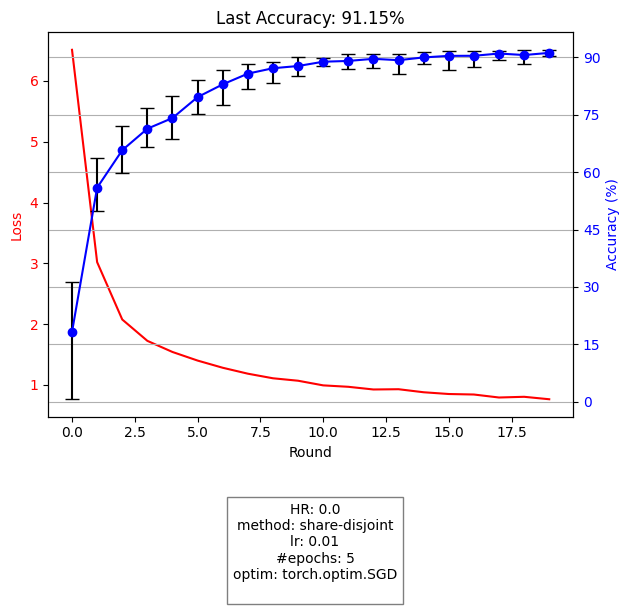
\includegraphics[width=\textwidth]{../plots/har-horizontal/sgd/results-h0_0-hm_share-disjoint-lr0_01-e5-torch_optim_SGD.png}
        \caption{0\% Condivisione}
        \label{fig:hars0sgd}
    \end{subfigure}
    \hfill
    \begin{subfigure}[b]{0.49\textwidth}
        \centering
        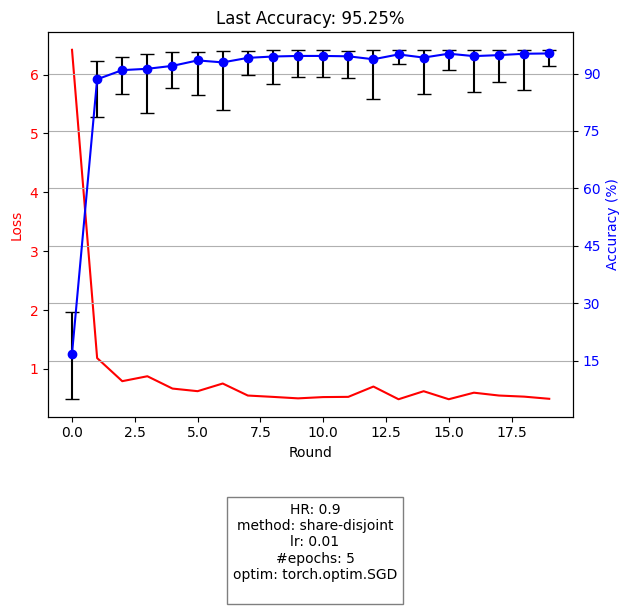
\includegraphics[width=\textwidth]{../plots/har-horizontal/sgd/results-h0_9-hm_share-disjoint-lr0_01-e5-torch_optim_SGD.png}
        \caption{100\% Condivisione}
        \label{fig:hars9sgd}
    \end{subfigure}
    
    \caption{
        Risultati del training per ogni round. A sinistra (a) si può 
        vedere l'apprendimento federato, a destra (b) quello centralizzato.
        Algoritmo di ottimizzazione (SGD) e metodo di condivisione 
        (\texttt{share-disjoint}) sono tenuti fissati.
    }
\end{figure}


Una differenza interessante rispetto al FEMNIST è che in questo 
caso AdamW si comporta sensibilmente meglio. Tanto per cominciare
le performance dei modelli allenati con SGD sono perfettamente 
comparabili a quelle dei modelli allenati con AdamW, anziché 
performare peggio. Inoltre AdamW mostra una maggiore resistenza 
all'instabilità dell'apprendimento provocata dalla condivisione 
dei dataset con il metodo \texttt{unify}. In figura 
\ref{fig:haru6sgd} si può vedere il risultato del training con SGD,
metodo \texttt{unify} al 60\% di condivisione, mentre in figura 
\ref{fig:haru6adam} si vede il risultato del training sotto le 
stesse condizioni usando l'algoritmo AdamW. Come si può vedere 
dagli intervalli di incertezza AdamW risulta più stabile in 
queste condizioni.
\begin{figure}[htp]  % h: here, t: top, b: bottom, p: page
    \centering
    \begin{subfigure}[b]{0.49\textwidth}
        \centering
        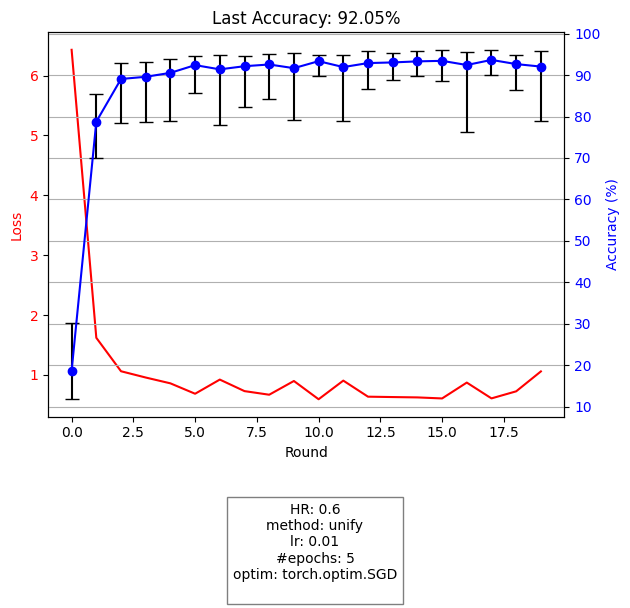
\includegraphics[width=\textwidth]{../plots/har-horizontal/sgd/results-h0_6-hm_unify-lr0_01-e5-torch_optim_SGD.png}
        \caption{Training con SGD}
        \label{fig:haru6sgd}
    \end{subfigure}
    \hfill
    \begin{subfigure}[b]{0.49\textwidth}
        \centering
        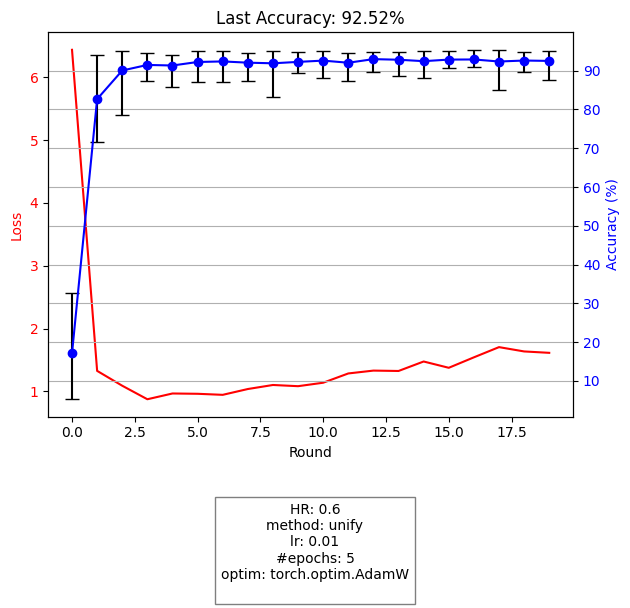
\includegraphics[width=\textwidth]{../plots/har-horizontal/adam/results-h0_6-hm_unify-lr0_01-e5-torch_optim_AdamW.png}
        \caption{Training con AdamW}
        \label{fig:haru6adam}
    \end{subfigure}
\end{figure}

Concludendo quest'analisi, anche in questo si è potuto riscontrare
un effettivo miglioramento di performance all'aumentare dell'ibridazione,
seppur con margini più stretti, in quanto l'accuracy del modello 
federato è già piuttosto alta. Passando da condivsione nulla ad allenamento
centralizzato si ottiene un miglioramento complessivo di circa 5 punti 
percentuali. Anche in questo caso con una condivisione del 20\% si può 
ottenere la maggior parte di questo miglioramento e con una condivisione 
del 40\% si ottengono risultati davvero simili a quelli del modello 
centralizzato (94.5\% contro un 95.25\% per il centralizzato).

Tutti i grafici degli esperimenti sull'UCI HAR sono nell'appendice B

\clearpage
\section{HAR - VFL}
L'ultimo esperimento fatto è quello del UCI HAR con partizionamento 
verticale delle feature.

In questo caso la rete neurale che compie la classificazione è 
distribuita tra client e server. Dato un numero di client \(K\) 
configurabile ogni ogni client ha un MLP che accetta \(561 / K\)
feature (dove l'utlimo client prende le feature rimanenti in caso di 
resto diverso da 0) e ne calcola un encoding. Sono state provate due 
dimensioni diverse di encoding: su un vettore lungo 10 e lungo 100.
Data la lunghezza \(l\) del vettore di encoding, il server ha un'altra 
MLP che accetta un vettore lungo \(Kl\) e ne calcola la classificazione.
Sia il modello dei client che quello del server hanno un hidden layer 
di 50 neuroni.

I risultati di questo esperimento sono stati però deludenti: a discapito
di quale ottimizzatore venisse utilizzato tra SGD e AdamW, del numero di client da 
3 a 50 e della dimensione dell'encoding non si è mai riusciti ad ottenere 
un'accuracy superiore al 18\%, rimanendo quindi appena sopra
1 / 6 = 16.7\% cioè la probabilità di prenderci tirando a caso ogni 
volta su 6 classi. Si può quindi concludere che questo partizionamento
delle feature su questo dataset non è un approccio funzionante.


\section{Possibili sviluppi futuri}
Come già accennato, questo studio non ha l'obbiettivo di ottenere le 
migliori prestazioni possibili e come tale offre un ampio margine di 
miglioramento, specie nel caso in cui queste stesse tecniche vengano 
applicate a problemi più complessi.  


\subsubsection{Funzioni di attivazione}
Un primo possibile miglioramento 
è quello di cambiare alcuni parametri 
della rete neurale.
La funzione di attivazione ReLU, ad esempio, è 
estremamente popolare ed efficace nel mitigare il problema del 
vanishing gradient, ma anch'essa ha le sue limitazioni come il 
problema del \textit{dying ReLU}. Alternative che possono essere 
esplorate sono la Leaky ReLU (LReLU) ~\cite{Maas2013RectifierNI},
definita come
\[
LReLU(z) = 
\begin{cases} 
      z, & \text{se } z > 0 \\
      \alpha z, & \text{altrimenti}
\end{cases}
\]
che ammette valori diversi da 0 per argomenti negativi e introduce un 
altro iperparametro \(\alpha\), tipicamente piccolo,
o la Parametric ReLU (PReLU) che rende l'iperparametro \(\alpha\)
un parametro \(a_i\) da imparare per ogni neurone:
\[
PReLU(z_i) = 
\begin{cases} 
      z_i, & \text{se } z_i > 0 \\
      a_i z_i, & \text{altrimenti}
\end{cases}
\]
Altre varianti della ReLU interessanti, in quanto funzioni liscie e 
differenziabili anche su 0, sono la Gaussian Error Linear Units (GELU)
~\cite{hendrycks2016gelu}
\[
GELU(z) = z P(Z \le z) = z \Phi(z)
\]
o la Exponential Linear Unit (ELU) ~\cite{clevert2016elu}, 
che assume anche valori negativi fino a -1
\[
ELU(z) = 
\begin{cases} 
      z, & \text{se } z > 0 \\
      \alpha (e^z - 1), & \text{altrimenti}
\end{cases}
\]
per un qualche iperparametro \alpha < 0.


\subsubsection{Regolarizzazione}
In questi esperimenti non si è fatto particolare uso di tecniche di 
normalizzazione o regolarizzazione, se non per una normalizzazione 
applicata alla immagini del FEMNIST ottenuta dalle trasformazioni 
built-in fornite da PyTorch. Si potrebbe allora provare alcune di 
queste tecniche come l'utilizzo della normalizzazione \(L_2\) in caso si 
usi SGD (\(L_2\) e weight decay sono equivalenti solo sotto SGD 
~\cite{Loshchilov2017AdamW}) oppure una delle varie tecniche di 
normalizzazione che velocizzano il training riducendo l'effetto del 
\textit{covariate shift}, come la batch normalization ~\cite{ioffe2015batch},
la layer normalization ~\cite{ba2016layer} o la group normalization 
~\cite{wu2018group}


\subsubsection{Scaling Up}
Un altro metodo efficace per migliorare le performace di una rete neurale 
è quello di scalare le dimensioni del modello, dei dataset o del training.
Operare con un'ampia mole di utenti e quindi con molte fonti di dati,
far produrre più dati per il training ove possibile o rendere i modelli 
più complessi possono essere opzioni percorribili. Bisogna tenere in 
considerazione il fatto che modelli più grandi possono incappare nel 
problema dell'overfitting, richiedere più risorse computazionali, 
rischiando di tagliare fuori alcuni dispositivi meno performati, e 
aumenta l'utilizzo della banda di rete per la comunicazione di un 
maggior numero di parametri.


\subsubsection{Inductive Bias migliori}
Un'altra recente area di studio nel campo del deep learning è quella 
della ricerca di architetture che per come sono costruite implementano
strutturalmente un'invarianza desiderata a qualche trasformazione 
dell'input. Un esempio concreto è l'invarianza traslazionale che 
implementano i layer convoluzionali attraverso la condivisione dei pesi.
Il geometric deep learning ~\cite{bronstein2021geometric} è lo studio di simmetrie 
(i.e. invarianti o equivarianti) geometriche che possono essere sfruttate nella 
progettazione di architetture neurali.
Il FEMNIST è un dataset particolare in cui tutti i caratteri sono stati
centrati e riscalati per ricoprire tutti la stessa area, cosa che in 
generale nella scrittura naturale è lontana dalla realtà. Può essere 
interessante esplorare architetture convoluzionali che siano invarianti 
anche a rotazioni o rescaling ~\cite{sosnovik2023symmetry, cohen2016group,
marcos2016rotation, cohen2016steer}.

Rimane però il fatto che le simmetrie desiderate dipendono fortemente 
dal problema trattato e per tale ragione vanno analizzate per lo 
specifico problema preso in considerazione.


\subsubsection{Data Augmentation}
Un altro metodo per \textit{insegnare} ad un modello ad essere invariante
a certe trasformazioni come la rotazione è quello del data augmentation.
In questo caso quello che si può fare è produrre nuovi dati da fornire
al modello nel training, facendo delle trasformazioni sui dati 
originali (come appunto rotare le immagini, aggiungere noise artificiale,
invertire le immagini...) o anche producendo dati sintetici del tutto
nuovi. Nell'era dei modelli generativi infatti, un'ulteriore possibilità
è quella di far generare dei dati del tutto sintetici ad un modello 
generativo che abbiano la stessa distribuzione dei dati naturali.

Bisogna però tenere presente che questo approccio non è efficace nel 
risolvere il problema della \textit{curse of dimensionality}
~\cite{bellman1957dynamic, Hughes1968OnTM, bronstein2021geometric}, 
per cui il numero di data points nel training set scala esponenzialmente 
in funzione della dimensionalità dell'input della funzione che 
cerchiamo di apprendere.
